
\chapter{Memory matters}
\label{ch:memoryMatters}

This chapter is near and dear to my heart. The concepts here are vastly
undertaught by computer science educators today, and yet they are at the
epicenter of most intermediate students' understanding (or misunderstanding).
A failure to master this material slaps a hard ceiling on what you can
accomplish as a programmer. Successfully mastering it is the key to the next
level.

The key idea is that there are two ways of looking at a computer program. One
is to look at the static lines of code as they are written on a screen or on
paper. This is how novices think about programs: they look at the lines of
code, and ask themselves whether lines need to be added, removed, changed, or
moved.

\index{memory}
The other way is to think about what happens to the computer's \textbf{memory}
as the program runs, and how its variables and structure change as the program
unfolds. Whether they realize it or not, this is how all proficient
programmers think. It turns out that \textbf{the ``purpose'' of almost any line
of code is to change the contents of memory in a particular way.} The name of
the game is recognizing what impact on memory each line of code has -- and
conversely, what line of code is required to make a particular change to
memory.

\section{Memory diagrams}

\index{memory diagram}
\index{snapshot}
The focal point of this chapter will be the \textbf{memory diagram}, which
incorporates the UML object representations we discussed in
section~\ref{sec:UMLclasses}. A memory diagram depicts the contents of the
computer's memory at a \textit{snapshot in time.} At any given moment, as a
program is running, you could say ``Freeze!''\ and look at the memory diagram.
It would give you the exact state of the system at that moment.

\subsection{The stack and the heap}

\index{stack@the stack}
\index{heap@the heap}
\index{memory!statically-allocated}
\index{memory!dynamically-allocated}
A program's memory, it turns out, is divided into two realms with funny names:
``\textbf{the stack}'' and ``\textbf{the heap}.'' It is vital to understand the
difference between the two, and which one is used for what. The stack contains
\textbf{statically-allocated} memory and the heap contains
\textbf{dynamically-allocated} memory. We'll unpack what all this means, but
first let me show you a full list of differences:

\vspace{.2in}
\begin{tabular}{c|c}
\textbf{stack} & \textbf{heap} \\
\hline
statically-allocated & dynamically-allocated \\
\index{names}
contains named things & contains unnamed things \\
contains primitive types and references & contains objects\footnote{This is
true in Java, but C++ permits programmers to store objects on the
\textit{stack} as well as the heap. I will argue that's universally dumb, and
that is a large part of what makes programming in C++ difficult: you have to
account for that happening, which requires a ton of tedious and error-prone
bookkeeping.} \\
\index{lifespan}
items have a limited lifespan & items have an unlimited lifespan\footnote{Not
completely unlimited, but things on the heap stick around as long as they're
needed, rather than evaporating at the end of their current function.} \\
\end{tabular}
\vspace{.2in}

This is best understood by example, and in fact can be illustrated with just a
small function:

\begin{figure}
\begin{Verbatim}[fontsize=\small,samepage=true,frame=single]
void illustration() {
    int year = 2018;
    Car minivan = new Car("Toyota","Sienna");
}
\end{Verbatim}
\caption{Some surprisingly complex code.}
\label{fig:firstCode}
\end{figure}

This teensy function, when it runs, produces memory contents as depicted in
Figure~\ref{fig:stackHeap1}. Let's go through it carefully.

\begin{figure}   % 590x220
\centering
\includegraphics[width=1\textwidth]{stackHeap1.pdf}
\caption{The stack and the heap.}
\label{fig:stackHeap1}
\end{figure}

\index{primitive type}
The first line of \texttt{illustration()} creates a simple integer variable
and sets it equal to 2018. Since an \texttt{int} is a \textbf{primitive
type}\footnote{If you've never heard this lingo, a ``primitive type'' is one of
the very basic lower-case Java variable types, like \texttt{int},
\texttt{double}, or \texttt{boolean}. Importantly, a primitive type is
\textit{not} an object.}, it is stored on the stack. ``On'' the stack should
make you think of layering items vertically on a surface. Before this line of
code executed, nothing existed in the program's memory at all, so the stack
was nothing but a bare floor (think of it as a horizontal line). Our first
variable goes right on top of that floor.

\index{reference variable}
\index{variable, reference}
There's a ton packed into that second line of code, so hold on to your seats.
The first thing to realize is that \textit{it encompasses both stack and
heap.} We have a named \textbf{reference variable} called \texttt{minivan},
which, as with all named things, goes on the stack (right on top of
\texttt{year}). A ``reference variable'' means a variable that has the ability
to reference (or ``refer to,'' or ``point to'') an object. However, the object
itself is created in the heap, because in Java that's where all objects live.
The word \texttt{new} is a ``heap word'': using it is the only way to make an
object at all, and therefore, the only way to make something on the heap.
Finally, to carry out the equals sign (``\texttt{=}'') in that line of code, we
draw an arrow from \texttt{minivan} to the object to indicate that's what it's
currently referring to.

%\subsubsection{(...a brief commercial...)}
%
%Now before we go any further, I want to \textit{\textbf{implore}} you that
%\textit{this stuff does actually matter.} It's tempting at this point to think
%that all this gibberish about stack and heap and whether something's on the
%left or right side of a diagram is irrelevant.  Nothing could be further from
%the truth. As soon as our example gets even moderately complicated, you will
%absolutely get the wrong answer if you conflate or confuse the two memory
%realms, or fail to keep their contents utterly in sync. Trust me on this.
%
%\subsubsection{(...okay, back to work...)}

\index{names}
Okay, now a head-scratcher. Look at Figure~\ref{fig:stackHeap1} again. What
would you answer if I asked you, ``what's the \textit{name} of that blue
object?''

If you're like 99\% of novice programmers (including myself, long ago), you
would confidently answer, ``\texttt{minivan}. Its name is \texttt{minivan}.''
That seems to make perfect sense. But unfortunately it is \textit{wrong}. The
truth is that \textit{the object has no name.}

Again, you may think I'm being pedantic. Let me demonstrate why I'm not.
Suppose we expanded our previous code with four more lines:

\begin{figure}
\begin{Verbatim}[fontsize=\small,samepage=true,frame=single]
void illustration() {
    ...
    Car other = new Car("Ferrari","F355");
    Car t = minivan;
    minivan = other;
    other = t;
}
\end{Verbatim}
\caption{(Continuing the previous example.)}
\label{fig:additionalCode}
\end{figure}

\index{car@\texttt{Car}}
Let's deal with the first two of these lines. The first one creates a new
reference variable called \texttt{other} on the stack, and points it to a
brand new \texttt{Car} object (unrelated to our Toyota Sienna) in the heap.
Notice that unlike with the stack, I didn't carefully put the new \texttt{Car}
exactly on top of the first one. Instead, I just threw it in there helter
skelter. This is how the heap works, and in fact why it's called a ``heap'':
it's a disorganized mess of stuff that comes and goes in response to the
program's unpredictable needs. The stack is as tidy as the Library of
Congress; the heap is a teenage boy's room. Seems weird, but it turns out
things have to be that way.

The second line creates a new stack variable called \texttt{t} but
emphatically does \textit{not} create a new \texttt{Car} object. Let that sink
in deeply. Many programmers, upon seeing a line begin with ``\texttt{Car t =
...} would naturally assume that line is making a new \texttt{Car}. But it's
actually only creating another variable that has the \textit{potential} to
refer to a \texttt{Car}. And in fact, after the equals sign, we do point it to
a \texttt{Car}...but one of the ones we've already instantiated (namely, the
Sienna).

The result of executing these two lines is shown in
Figure~\ref{fig:stackHeap2}. Stare very carefully at that figure and mull over
each box and line. We have four named variables, three of which are of type
\texttt{Car}, and yet there are only \textit{two} \texttt{Car} objects because
we only executed two \texttt{new}'s. And two of our named variables --
\texttt{t} and \texttt{minivan} -- are pointing to \textit{the same object}.
This turns out to be okay. We'll have multiple references to the same object
all the time, and it's entirely healthy. What's critical not to miss is that
\texttt{t} and \texttt{minivan} are not referring to identical copies of the
\texttt{Car}, but literally \textit{the same \texttt{Car}}. If we were to
change the state of \texttt{t}'s \texttt{Car} by, say, increasing its odometer
instance variable, \texttt{minivan} would instantly experience the same
change. And that's because they \textit{are} the same. 

\begin{figure}
\centering
\includegraphics[width=1\textwidth]{stackHeap2.pdf}   % 620x230
\caption{After executing the first two lines of code
listing~\ref{fig:additionalCode}.}
\label{fig:stackHeap2}
\end{figure}


Okay, now the punchline of this whole example. I'm going to complete the
bait-and-switch, just to prove I was right before when I said ``the name of
that first blue box is \textit{not} \texttt{minivan}.'' Let's do the
\textit{second} two lines of code in listing~\ref{fig:additionalCode}:

\begin{Verbatim}[fontsize=\small,samepage=true,frame=single]
    ...
    minivan = other;
    other = t;
\end{Verbatim}

The result of those two operations is to change what the \texttt{other} and
\texttt{minivan} variables are pointing to. Memory now looks like
Figure~\ref{fig:stackHeap3}. And so I ask you again: ``what's the
\textit{name} of that Toyota Sienna object?'' I think you'll agree that
\texttt{minivan} is most certainly \textit{not} its name. Two valid ways to
refer to it are \texttt{t} and \texttt{other}, both of which point to it. But
neither one is its name. Objects simply have no name.

Names are ephemeral, momentary: they're only used temporarily so we can get at
the stuff in the heap, which is ultimately what matters.

\begin{figure}
\centering
\includegraphics[width=1\textwidth]{stackHeap3.pdf}   % 620x230
\caption{Finally, after executing the rest of code
listing~\ref{fig:additionalCode}.}
\label{fig:stackHeap3}
\end{figure}

\index{lifespan}
Let me conclude this example by explaining what I meant earlier about
``limited lifespans.'' After executing the ``\texttt{other = t;}'' line, we are
done with the function. It's time to return control to whoever called
\texttt{illustration()} in the first place. And at this point, all of our
named variables -- \texttt{t}, \texttt{other}, \texttt{minivan}, and even
\texttt{year} -- cease to exist. Their destiny was only to provide service
during the time that \texttt{illustration()} was being executed. 

But the stuff on the heap lives on after. Long after a function is completed,
the objects it may have created or changed have a presence that will affect
the behavior of other, future functions. In this case, since we weren't passed
any arguments and didn't return anything, our Toyota and Ferrari \textit{will}
actually peacefully go away. But in general there are meaningful, long-term
effects, and in the next section we'll see an example in action.

Most methods are just like this. They create a few named variables so they can
change the contents of the heap in some way, and then clean up their toys
and return with the heap thus changed. That is their \textit{raison d'etre}.
It's a short but happy life.


\section{Calling functions}

\index{function}
One thing our previous example didn't include was calling a function or
method. In this section, we'll see what happens to memory when we do this.
There will probably be a few eye-openers for you.

First, take a look at our code listing (Figure~\ref{fig:functionCode}). We'll
switch from an automotive domain to part of a baseball simulator.

\index{ballplayer@\texttt{Ballplayer}}
\begin{figure}
\centering
\begin{Verbatim}[fontsize=\footnotesize,samepage=true,frame=single]
class Simulator {
    public static void main(String args[]) {
        int year = 2018;
        String greeting = "Play ball!";
        Ballplayer oldGeezer;

        ArrayList yankees = buildDaTeam();
        int rosterSize = yankees.size();
    }

    static ArrayList buildDaTeam() {
        String name = "Yankees";
        int year = 1927;
        ArrayList team = new ArrayList();

        Ballplayer ruth = new Ballplayer("Babe Ruth");
        ruth.setUni(3);
        ruth.setPos("OF");
        Ballplayer gehrig = new Ballplayer("Lou Gehrig");
        ruth.setUni(4);
        ruth.setPos("1B");
        Ballplayer babe = ruth;
        babe.setUni(3);       // (Pointless, as it turns out.)
        babe.setPos("OF");    // (Pointless, as it turns out.)
        team.add(babe);
        team.add(gehrig);
        team.add(ruth);
        
        return team;
    }
}
\end{Verbatim}
\caption{Some code that calls a function.}
\label{fig:functionCode}
\end{figure}

Let's see how the memory diagram emerges line-by-line in response to the code
executing.

First, let's execute the first three lines of \texttt{main()} and
``Freeze!''\ the picture. The result of these lines is shown in
Figure~\ref{fig:bpStackHeap1}. There are three new things here worth
mentioning. First, notice that our \texttt{greeting} variable, although it is
a \texttt{String}-with-a-capital-S and therefore an object, is shown on the
\textit{stack}, just like the \texttt{int year} is. The reason for this is
that Strings are a kind of in-between case (between primitive types and
objects) -- they're neither fish nor fowl. Technically they're objects, but
Java actually treats them somewhat specially, and even has an inline syntax to
create what are actually instances, so it ends up making more sense to treat
them as primitive types on the stack. That's what we'll always do with
\texttt{String}s.

\begin{figure}   % 650x240
\centering
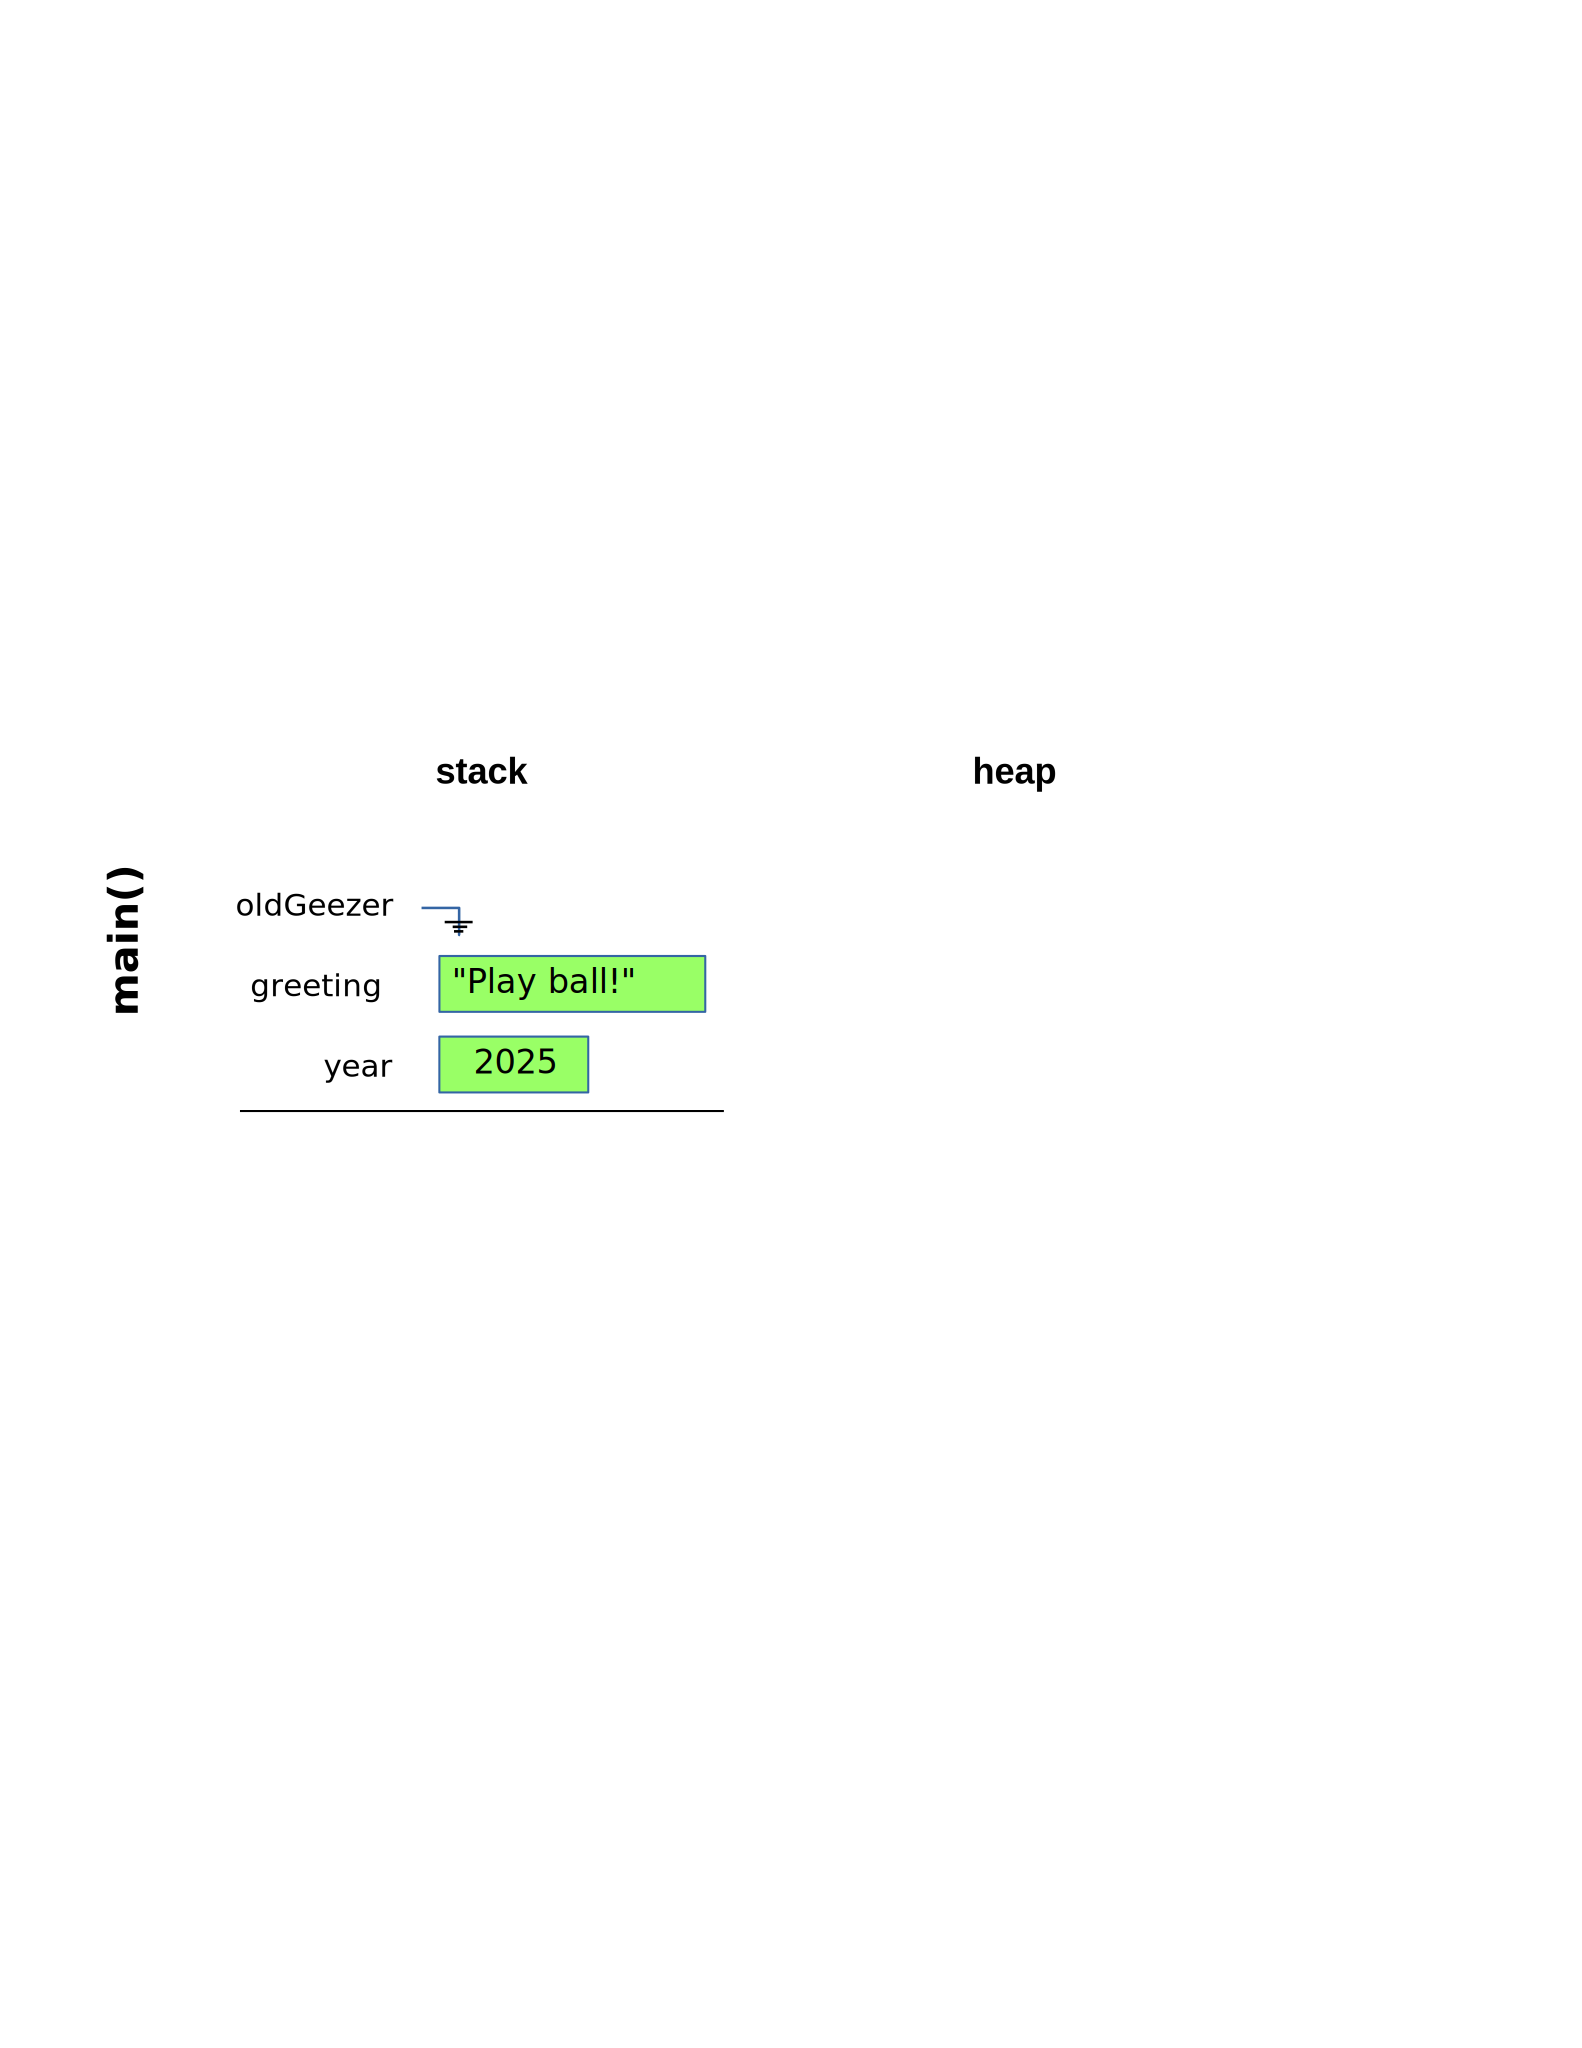
\includegraphics[width=.9\textwidth]{bpStackHeap1.pdf}
\caption{Memory contents after executing the first three lines of
\texttt{main()}.}
\label{fig:bpStackHeap1}
\end{figure}

\subsubsection{Null references and NPEs}

\index{null pointer (or reference)}
\index{null@\texttt{null}}
The next new thing is that bizarre symbol next to \texttt{oldGeezer}.
\textit{Whazzat?} If you look at the code listing, you'll see that we
declare a variable of type \texttt{Ballplayer} named \texttt{oldGeezer}, but
we never set it equal to a \texttt{new} instance, nor to anything else for
that matter. This means that \texttt{oldGeezer}, which as you'll recall is a
``reference variable'' (capable of referring to a \texttt{Ballplayer})
currently refers to \textit{nothing}. In Java, this is called a \textbf{null
reference} (or \textbf{null pointer}) and is indicated with the keyword
\texttt{null}. In fact, this line of code has exactly the same effect as the
one above:

\begin{Verbatim}[fontsize=\small,samepage=true]
    Ballplayer oldGeezer = null;
\end{Verbatim}

Some people prefer to be explicit like this. I don't care either way; just
realize that at this point, if you attempted to call \textit{any} method on
\texttt{oldGeezer}, like:


\begin{Verbatim}[fontsize=\small,samepage=true]
    Ballplayer oldGeezer = null;
    oldGeezer.strikeout();
\end{Verbatim}

\index{NPE (null pointer exception)}
you will then be hit with the most ubiquitous of all Java
run-time errors, the \textbf{null-pointer exception} (or ``\textbf{NPE}''):

\begin{Verbatim}[fontsize=\small,samepage=true]
Exception in thread "main" java.lang.NullPointerException
    at Simulator.main(Simulator.java:5)
\end{Verbatim}

This is quite reasonable behavior, if you think about it. What can Java do if
you try to ``call a method on an object'' but there \textit{is} no such object?
It can only throw up its hands, which it does here.

Remember: an NPE means \textit{you tried to call a method on an object, but
the variable name you called it on wasn't actually an object; it was}
\texttt{null}. The way to diagnose an NPE is to look at the line number it
gives you, and find the dot (``\texttt{.}'') (or dots) on that line. The
variable or expression to the \textit{left} of one of those dots is an
uninitialized, null reference. Guaranteed.

\subsubsection{Stack frames}

\index{stack frame}
\index{recursion}
The last new thing in Figure~\ref{fig:bpStackHeap1} is easy to miss: it's the
word \texttt{main()} off on the left-hand side of the diagram. What this means
is that \textit{all the variables to the right of it ``belong'' to the
\texttt{main()} function.} This group of variables, which goes with a
particular call to a function\footnote{Note carefully that a stack frame is
associated with each \textbf{\textit{call}} to a function, not each function.
This may seem pedantic, and it is...until we consider \textbf{recursion}. A
recursive function will call itself, which will call itself, which will call
itself...many times. \textit{Each call} to the function generates its own
stack frame, which is separate from all the others. This is how recursive
functions are able to work without clobbering the values of the variables
contained in previous, still-active calls.}, is called a \textbf{stack frame}.
The way a program works is this: every time a function is called, a new stack
frame is ``pushed'' on top of the stack (above a horizontal line that we'll
draw.) While we're in the function, \textit{Java can only see the variables in
that current stack frame.} The ones in \texttt{main()}'s stack frame, or any
other stack frame for currently-in-progress functions, are safely nestled away
to be resumed later, but they are not immediately available to the program.

This is exactly how it should be. If we call a function \texttt{foo()} from
within a function \texttt{bar()}, control transfers to \texttt{foo()}. Now how
could \texttt{foo()} possibly refer to \texttt{bar()}'s variables? Heck,
whoever wrote the code for \texttt{foo()} didn't even know it would be
\textit{called} from \texttt{bar()}! Any other function could have called it
just as well, in which case \texttt{bar()}'s variables wouldn't even exist.
All we know for sure is that \texttt{foo()} was called from ``somewhere,'' and
thus must work no matter what the context. If Java allowed us to talk about
variables in another stack frame, our function would instantly become
non-reusable; it would only make sense if called from some specific other
function. And that defeats most of the purpose of even having a function.

Okay, now the big moment. We run this line:

\index{buildDaTeam@\texttt{buildDaTeam()}}
\begin{Verbatim}[fontsize=\small,samepage=true]
        ArrayList yankees = buildDaTeam();
\end{Verbatim}

which calls the \texttt{buildDaTeam()} function and transfers control to it.

Hang on to your hats. A lot happens here. First, a \textit{new stack frame} is
created, labeled \texttt{buildDaTeam()} in the diagram to carefully
distinguish it from the other. Then, \texttt{buildDaTeam()} starts executing.
Let's do the first three lines. We create two new variables on the stack
(a \texttt{String} and an \texttt{int}). One of these (\texttt{year}) has
\textit{the same name} as a variable that was declared down in
\texttt{main()}. This is perfectly okay, and the two \texttt{year}s in fact
have nothing whatsoever to do with each other. As long as
\texttt{buildDaTeam()} has control, ``\texttt{year}'' means \textit{the top
year}, in \texttt{buildDaTeam()}'s stack frame.

\index{null@\texttt{null}}
\index{instantiation}
In the third line, we create our first heap object of the entire program. It
is created (as all objects are created) with the \texttt{new} keyword. This
newly instantiated thing is an \texttt{ArrayList}, and we'll draw it as
indicated in Figure~\ref{fig:bpStackHeap2}. It has some \texttt{contents},
which is a zero-based, array-ish list of references, each of which has the
potential to point to an object.\footnote{You may be more used to seeing
\texttt{ArrayList<Ballplayer>} instead of just plain \texttt{ArrayList}, which
actually is a better choice. When we declare something as type
``\texttt{ArrayList<Ballplayer>}'' we're saying ``Java, please prevent me from
storing anything in this \texttt{ArrayList} \textit{except}
\texttt{Ballplayer}s.'' See section~\ref{sec:generics} for more details.}
Currently none of them do so, and therefore the diagram shows the
\texttt{null} symbol for each.

\index{snapshot}
Freeze! The program's memory now looks like Figure~\ref{fig:bpStackHeap2}.
Run your eyeballs over it and make sure you understand every box and line.

\begin{figure}   % 650x400
\centering
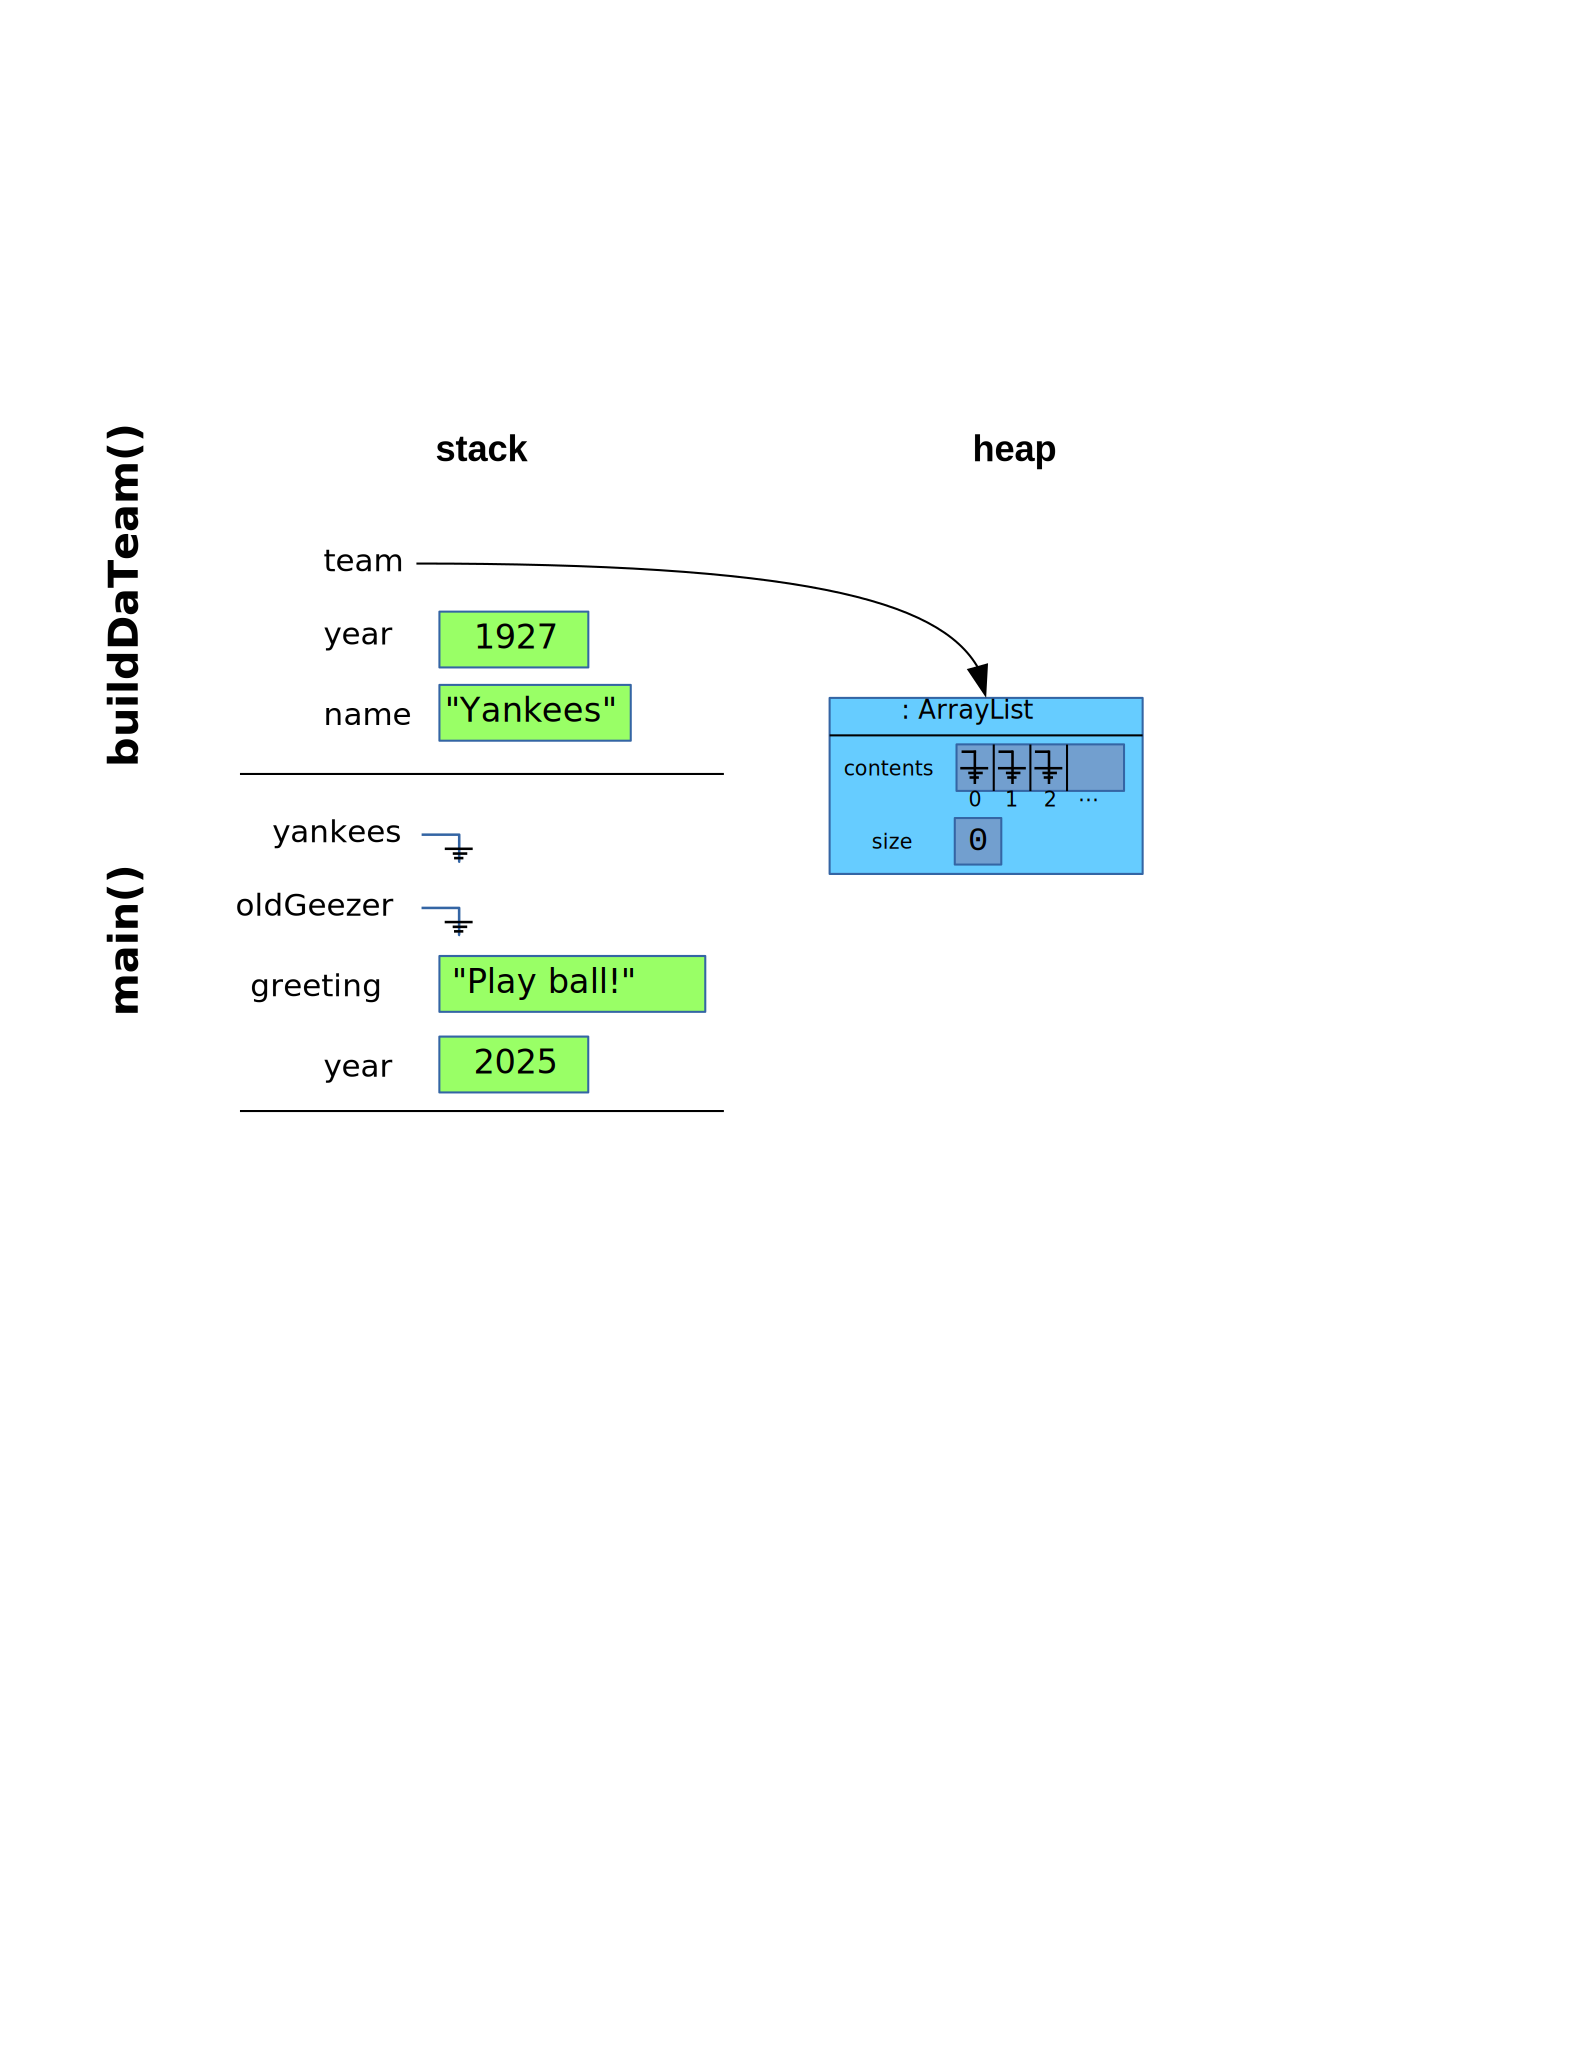
\includegraphics[width=.9\textwidth]{bpStackHeap2.pdf}
\caption{Memory contents after calling the function and executing the first
three lines of \texttt{buildDaTeam()}.}
\label{fig:bpStackHeap2}
\end{figure}

\subsubsection{Object craziness}

Now for the next part of code listing~\ref{fig:functionCode}. These three
lines:

\begin{Verbatim}[fontsize=\scriptsize,samepage=true,frame=single]
        ...
        Ballplayer ruth = new Ballplayer("Babe Ruth");
        ruth.setUni(3);
        ruth.setPos("OF");
        ...
\end{Verbatim}

\index{instantiation}
instantiate a new \texttt{Ballplayer} object (on the heap, of course) and set
it to some initial values. You need a little imagination to envision what the
\texttt{Ballplayer} class does in response to these method calls, but only a
little: obviously it has a constructor that takes a \texttt{String} (the
player's full name) and a couple of accessor/mutator methods to set the
player's uniform number and position. 

We then do the same sort of thing again, for another player:

\begin{Verbatim}[fontsize=\scriptsize,samepage=true,frame=single]
        ...
        Ballplayer gehrig = new Ballplayer("Lou Gehrig");
        gehrig.setUni(4);
        gehrig.setPos("1B");
        ...
\end{Verbatim}

to get another one. Then, we do this:

\begin{Verbatim}[fontsize=\scriptsize,samepage=true,frame=single]
        ...
        Ballplayer babe = ruth;
        babe.setUni(3);       // (Pointless, as it turns out.)
        babe.setPos("OF");    // (Pointless, as it turns out.)
        ...
\end{Verbatim}

\index{new@\texttt{new}}
which you know by now does \textit{not} instantiate a new object. (After all,
there's no \texttt{new}.) Instead, the first line \textit{points the new
variable \texttt{babe} at the same object \texttt{ruth} is currently pointing
to.} Get very, very comfortable with the idea that except for primitive types,
``\texttt{=}'' in Java does not do anything resembling a ``copy'' operation. It
simply makes a reference variable refer to something else. So we now have
three variables of type \texttt{Ballplayer}, but only \textit{two}
\texttt{Ballplayer} objects.

Finally, we add these players to our \texttt{ArrayList}:

\begin{Verbatim}[fontsize=\scriptsize,samepage=true,frame=single]
        ...
        team.add(babe);
        team.add(gehrig);
        team.add(ruth);
        ...
\end{Verbatim}

Stare closely at all those crazy arrows in Figure~\ref{fig:bpStackHeap3} and
make sure you understand where they're all going and why. Our
\texttt{ArrayList} object, instead of showing \texttt{null} pointers, now has
each of its slots pointing to a particular \texttt{Ballplayer} object.
Elements 0 and 2 point to the \textit{same} object, of course, because we
added ``\texttt{babe}'' and later ``\texttt{ruth}'' and those two variables are
pointing to the \textit{same} object. (So we're cheating here, baseball-wise:
you can't actually have the same player twice in the lineup! This is just an
example.)

\begin{figure}   % 800x460
\centering
\includegraphics[width=1\textwidth]{bpStackHeap3.pdf}
\caption{Memory after all the object creation done in \texttt{buildDaTeam()}.}
\label{fig:bpStackHeap3}
\end{figure}

\subsubsection{``I shall return''}

And now, we're ready to polish off this bad boy.

\begin{Verbatim}[fontsize=\scriptsize,samepage=true,frame=single]
        ...
        return team;
    }
\end{Verbatim}

\index{return@\texttt{return}}
That ``\texttt{return}'' statement packs a wallop. When the function is
completed, two huge things happen. First, the function's stack frame
\textit{is entirely wiped out.} Like, off the face of the planet. Every single
variable in there is irrevocably deleted and never mentioned again.

\index{stack@the stack}
\index{heap@the heap}
When students first hear this, they're sometimes dismayed -- ``what's the
point of calling a function then, if every single thing it creates is erased?''
Ahhhh...but they're only thinking of the \textit{stack}, not the heap. The
heap-ish things that a function accomplishes \textit{do} live on, and as I
said earlier, they are the reason the function existed in the first place.
Almost all functions' sole job is to inspect or manipulate the heap in some
way.

\index{stack frame}
When I say the stack frame is wiped out, here's what's wiped out: (1) all the
named variables in the stack frame, (2) all the primitive type values in the
stack frame (green boxes), (3) all the arrows emanating from the stack frame's
reference variables, (4) the word on the side of the diagram that names the
function, and even (5) the horizontal line that separates it from the stack
frame below.

\index{lifespan}
The result is that the top stack frame gets vaporized, leaving
\texttt{main()}'s stack frame open to the outside air. And that is exactly
what we want, because it's \texttt{main()}'s turn to take over now. Note that
all the heap stuff is still there: objects on the heap have an unlimited
lifespan, you'll remember.

\begin{figure}   % 750x460
\centering
\includegraphics[width=1\textwidth]{bpStackHeapFinal.pdf}
\caption{What memory looks like when we reach the end of \texttt{main()}.}
\label{fig:bpStackHeapFinal}
\end{figure}

\index{return@\texttt{return}}
The other thing the \texttt{return} statement does, of course, is put the
function's return value in the proper place, just before it's nuked. In this
case, since our original line of code was:

\begin{Verbatim}[fontsize=\scriptsize,samepage=true,frame=single]
        ArrayList yankees = buildDaTeam();
\end{Verbatim}

it makes \texttt{yankees} refer to the object that was ``returned,'' namely the
\texttt{ArrayList} that the shortly-to-die \texttt{team} variable is pointing
to.

We run one more line of code just to show we can do something with the
returned object (``\texttt{int rosterSize = yankees.size();}'') and the final
result is as in Figure~\ref{fig:bpStackHeapFinal}. There's no record of us
having called a function at all -- \texttt{buildDaTeam()} simply did its job
dutifully and quietly, and \texttt{main()} gets to reap the result.

\subsection{Calling a function from a function}

\index{function}
\index{stack frame}
By the way, this point is probably obvious by now, but let me clarify anyway:
if you call a function, and that function \textit{itself} calls
\textit{another} function, the same thing happens. The second function gets
its own stack frame with its own variables, while both the first function and
\texttt{main()} both get put on pause. There are at that moment \textit{three}
stack frames. When the second function returns, its stack frame disappears and
the first function becomes active; and when the first function returns,
\textit{its} stack frame disappears and \texttt{main()} becomes active.

\index{stack@the stack!pushing on}
\index{stack@the stack!popping off}
The terminology we use to describe this is somewhat obscure: when we create a
new stack frame for a newly-called function we call it \textbf{pushing} a new
frame on the stack. When we return, and get rid of it, we call it
\textbf{popping} the frame off the stack. Push and pop are lingo you'll see in
Data Structures class, when a data structure called a ``stack'' is introduced.
That stack data structure is a more general category of memory management
technique, of which ``the stack'' of our present chapter is an example.

Anyway, this whole push-a-frame-every-time-you-call-a-method thing (and
pop-the-top-frame-every-time-you-return thing) is central to how any computer
program operates. It's how your program breathes.


\section{Calling methods}

\index{method}
\index{this@\texttt{this}}
The mechanics of calling a function are just the same as when calling a
method, except for one thing: \texttt{this}. It turns out that when you call a
method on an object, you're adding one more thing to the stack: a reference to
the object the method was called on. And that, of course, is precisely what
``\texttt{this}'' means.

\index{ballplayer@\texttt{Ballplayer}}
\index{batting average}
Let's pan over to a different part of our fictitious baseball simulator: the
\texttt{Ballplayer} class itself. Part of the code for it is in
Figure~\ref{fig:BallplayerCode}.\footnote{Apologies to non-baseball fans. All
you really need to understand this example is that in baseball, every batter
accumulates a number of ``at bats'' (chances to come to the plate and hit
against a pitcher) and a number of ``hits'' (times he/she actually hit the ball
and made it at least to first base). A player's ``batting average'' is the hits
over the at bats; it ostensibly tells you how likely (on a scale of 0 to 1)
that player is to get a hit if he/she bats.}

\begin{figure}
\begin{Verbatim}[fontsize=\scriptsize,samepage=true,frame=single]
class Ballplayer {
    String name, position;
    int uni, numHits, numAtBats;

    Ballplayer(String name) {
        this.name = name;
        numHits = 0;
        numAtBats = 0;
    }

    void strikeout() {
        numAtBats++;
    }

    void getAHit() {
        numHits++;
        numAtBats++;
    }

    double getBattingAverage() {
        return ((double) numHits)/numAtBats;
    }
    ...
}
\end{Verbatim}
\caption{Part of the \texttt{Ballplayer} class.}
\label{fig:BallplayerCode}
\end{figure}

\index{pitcher@\texttt{Pitcher}}
\index{face@\texttt{.face()}}
\index{KO (strikeout)}
We're going to have a different class for pitchers, since they have different
stats (see Figure~\ref{fig:PitcherCode}).\footnote{Here, we're going to model
each pitcher as having a ``\texttt{koDominance}'' (``KO'' is baseball lingo for
``strikeout,'' btw). This is a number between 0 and 1 indicating the
probability of overwhelming the batter with a strikeout without that batter
being able to do anything about it.} The only method we'll show on the
\texttt{Pitcher} class is \texttt{.face()}, which is where a pitcher ``faces''
(pitches to) a batter in our simulation. The result will either be strikeout
or a hit in our extremely simplified view of the baseball world.

\begin{figure}
\begin{Verbatim}[fontsize=\scriptsize,samepage=true,frame=single]
class Pitcher {
    String name, handedness;   // L or R
    int uni, numKos;
    double koDominance;        // between 0 and 1
    static java.util.Random rng = new java.util.Random();

    ...
    void face(Ballplayer batter) {
        double koRandNum = rng.nextDouble();
        double batterRandNum = rng.nextDouble();
        if (koRandNum < koDominance) {
            batter.strikeout();
            this.numKos++;
        } else {
            if (batterRandNum < batter.getBattingAverage()) {
                batter.hit();
            } else {
                batter.strikeout();
                numKos++;
            }
        }
    }
}
\end{Verbatim}
\caption{Part of the \texttt{Pitcher} class.}
\label{fig:PitcherCode}
\end{figure}

\index{static@\texttt{static}}
\index{random number generation}
\index{Random.nextDouble@\texttt{Random.nextDouble()}}
\label{Random}
One item of note is the \texttt{static} variable \texttt{rng}, which stands
for \textbf{r}andom \textbf{n}umber \textbf{g}enerator. It's an instance of
the \texttt{java.util.Random} class, which the Java API provides to roll
random numbers. Every time you call \texttt{.nextDouble()} on a
\texttt{Random}, it generates a new random number between 0 and 1. It makes
sense for this to be a \texttt{static} variable, since the random number
generator itself is an object that all objects will share and use.

\index{face@\texttt{.face()}}
The specifics of the \texttt{.face()} algorithm aren't important to
understand. What is important is what happens in memory as this method is
called. Let's say our \texttt{main()} has the code in
Figure~\ref{fig:showdownCode}. After executing all lines but the last one, we
have the picture in Figure~\ref{fig:pitcherStackHeap1}. Take a moment and
convince yourself it's correct in all details.

\begin{figure}
\begin{Verbatim}[fontsize=\small,samepage=true,frame=single]
    public static void main(String args[]) {

        Ballplayer joltinJoe = new Ballplayer("Joe Dimaggio");
        joltinJoe.setUni(5);
        joltinJoe.setPosition("OF");

        Ballplayer theSayHeyKid = new Ballplayer("Willie Mays");
        theSayHeyKid.setUni(24);
        theSayHeyKid.setPosition("OF");

        Pitcher bestOfAllTime = new Pitcher("Sandy Koufax");
        bestOfAllTime.setUni(32);
        bestOfAllTime.setHandedness("L");
        bestOfAllTime.setKoDominance(.5);

        bestOfAllTime.face(theSayHeyKid);
    }
\end{Verbatim}
\caption{A mighty showdown on the diamond.}
\label{fig:showdownCode}
\end{figure}

\begin{figure}
\centering
\includegraphics[width=1\textwidth]{pitcherStackHeap1.pdf}  % 750x350
\caption{The baseball simulator's memory immediately before executing the
\textit{last} line of \texttt{main()} (``\texttt{bestOfAllTime.face(theSayHeyKid)}'').}
\label{fig:pitcherStackHeap1}
\end{figure}


And now for the moment we've all been waiting for: the first pitch of a new
(fantasy) baseball season, in which Sandy Koufax, the greatest pitcher of all
time, will face down Willie Mays, quite possibly the greatest hitter of all
time. I can't stand the suspense!!

\begin{figure}
\centering
\includegraphics[width=1\textwidth]{pitcherStackHeap2.pdf}  % 750x450
\caption{Memory while on the last line of \texttt{.face()}.}
\label{fig:pitcherStackHeap2}
\end{figure}

Figure~\ref{fig:pitcherStackHeap2} shows how memory looks during this
thrilling matchup. We're inside the \texttt{Pitcher}'s \texttt{.face()}
method, and so it has its own stack frame as expected. But I want to draw your
attention to two crucial aspects of this diagram:

\begin{enumerate}
\itemsep.1em
\index{this@\texttt{this}}
\item First, notice we have a visitor. On the stack frame, in addition to the
other expected variables, is none other than ``\texttt{this}''. Realize that
\texttt{this} is really just a reference variable like any other. What does it
refer to? \textit{The object the method was called on}, of course. In this
case, it's Sandy Koufax. How do we know? Because when we called it, we didn't
just say ``\texttt{face(theSayHeyKid)}'' but
``\texttt{\textit{bestOfAllTime.}face(theSayHeyKid)}''. So the object that
\texttt{bestOfAllTime} refers to will be pointed to by \texttt{this} while
we're inside the method. Ponder this deeply.

\item Second, recognize that the \texttt{batter} argument -- which is a
reference variable of type \texttt{Ballplayer} -- is referring to the
\textit{same} object that \texttt{theSayHeyKid} is pointing to back in
\texttt{main()}. It is emphatically \textbf{\textit{not}} a copy of the
object. That's critical, because otherwise our \texttt{.face()} method would
have no way of updating Willie Mays' stats as a result of this
confrontation.\footnote{If you learned these terms in 220, this point can be
equivalently stated as follows: ``Java uses \textbf{pass-by-reference} for
objects, not \textbf{pass-by-value}.'' (Java \textit{does} use pass-by-value
for \textit{primitive types}, as we've seen: \texttt{int}s and such have their
own presence on the stack, and so are \textit{copied} from stack frame to
stack frame.)}

\end{enumerate}

Drum roll, please, before we hear the announcer: \textit{``...and it's a
scorching four-seam fastball from Koufax: swing and a miss, strike three!''}
The way the random numbers turned out in this example, Koufax was so
overpowering that he struck out Mays without the latter having a fighting
chance. (See how \texttt{koRandNum} was less than Koufax's
\texttt{koDominance}, so he blew him away without the \texttt{else} statement
coming into play -- \textit{i.e.}, without Mays' batting prowess even having a
chance to shine).

Don't worry, Willie: maybe you'll get one of your 660 lifetime home runs next
time you're up to bat. Console yourself with this: a different ``Willie'' Hall
of Famer (Willie Stargell) once quipped, ``trying to hit against Sandy Koufax
is like trying to drink coffee with a fork.''


\begin{figure}
\centering
\includegraphics[width=1.1\textwidth]{pitcherStackHeapFinal.pdf}  % 800x350
\caption{The final memory picture. Note the changed inst vars!}
\label{fig:pitcherStackHeapFinal}
\end{figure}

\index{pass-by-value}
\index{pass-by-reference}
The last diagram of the chapter, Figure~\ref{fig:pitcherStackHeapFinal}, shows
the situation when we return to \texttt{main()}. It's important not to miss
the main point here: both objects (\texttt{Pitcher} and \texttt{Ballplayer})
have their stats updated as a result of this showdown. If you're coming from a
language like C++, which passes objects by value, you might be raising your
eyebrows right about now. Get used to it. In Java, passing an object to a
function/method makes \textit{that exact object} available to the
function/method, not a copy. And certainly \texttt{this} is a reference to the
very object the method was called on, not a copy of it. This turns out to be
almost always what we want.


